% !TeX root = ../thesis.tex
\chapter{Tổ chức và tiêu chí thực nghiệm}
\label{chap:experiment}

\section{Dữ liệu và phạm vi đánh giá}
Thực nghiệm sử dụng CQADupStack với nhiệm vụ tìm những câu hỏi có quan hệ liên quan hoặc trùng lặp với truy vấn. Mỗi miền có kho câu hỏi riêng, tập truy vấn và nhãn liên quan tương ứng. Kho dữ liệu có sẵn khi truy xuất, còn nhãn được dùng theo vai trò huấn luyện hoặc đánh giá đã xác định. Việc cho hệ thống tiếp cận kho câu hỏi không đồng nghĩa cho phép sử dụng nhãn test để chọn cấu hình.

Toàn bộ quá trình đã sử dụng mười hai miền theo những vai trò khác nhau. Programmers và Unix được dùng trong giai đoạn đầu. Android, GIS, Mathematica và Webmasters được bổ sung trong vòng v3. Sáu miền này trở thành dữ liệu phát triển và huấn luyện của hệ cuối. English, Gaming, Physics, Stats, TeX và WordPress được giữ lại cho giai đoạn xác nhận v2 tại thời điểm chốt giao thức. Số lượng dữ liệu và vai trò được tổng hợp trong Bảng~\ref{tab:data}.

\begin{table}[htbp]
\centering\small
\caption{Phạm vi dữ liệu trong các phép đánh giá của hệ cuối.}
\label{tab:data}
\begin{tabularx}{\textwidth}{@{}p{29mm}Yrr@{}}
\hline
\textbf{Vai trò} & \textbf{Các miền} & \textbf{Truy vấn} & \textbf{Tài liệu}\\\hline
Phát triển và huấn luyện & Programmers, Unix, Android, GIS, Mathematica, Webmasters & 4.842 & 174.303\\
Xác nhận chất lượng & English, Gaming, Physics, Stats, TeX, WordPress & 8.303 & 282.896\\
Đo online & Programmers, Unix & 1.948 & 79.558\\
\hline
\end{tabularx}
\source{Thực nghiệm của nhóm; tập online là một phần của nhóm miền phát triển}
\end{table}

Các phương pháp được đánh giá trên cùng phiên bản dữ liệu và nhãn liên quan, với cách xử lý câu hỏi nhất quán. Kết quả không bao gồm chính câu hỏi đang làm truy vấn. Đối chứng BM25 cũng được giữ cố định, bởi những khác biệt trong cách áp dụng BM25 có thể ảnh hưởng phép so sánh \cite{bm25_variants2020}. Những điều kiện chung này giúp kết quả phản ánh khác biệt giữa các phương pháp trên cùng một bài toán.

Cách gọi sáu miền xác nhận là ``mới'' mang ý nghĩa lịch sử tại thời điểm đóng băng. Sau khi thực nghiệm kết thúc, tất cả mười hai miền đã được xem xét trong quá trình nghiên cứu. Nếu nhóm tiếp tục đổi thuật toán dựa trên các kết quả này, sáu miền đó không còn là tập xác nhận chưa dùng cho lựa chọn mới. Phân biệt này cần thiết để không mở rộng mức bằng chứng của giao thức ban đầu sang một phiên bản tiếp theo.

\section{Phân chia dữ liệu và quy trình nghiên cứu}
Các truy vấn được chia thành năm phần, trong đó những câu hỏi có quan hệ gần được giữ cùng nhóm. Các phần dữ liệu lần lượt đảm nhận vai trò học, lựa chọn phương án và đánh giá; mỗi truy vấn được đánh giá đúng một lần trên phần dành riêng cho nó. Cách tổ chức này nhằm hạn chế việc các câu hỏi quá giống nhau xuất hiện ở cả phía phát triển và phía đánh giá, từ đó làm kết quả tốt hơn khả năng áp dụng thực tế.

Trong phát triển v2, nhóm lần lượt giữ riêng từng miền để xem bộ quyết định học từ các miền còn lại có tiếp tục hữu ích hay không. Kết quả trung bình theo miền được dùng để lựa chọn phương án và ngân sách. Sau đó, bộ quyết định được học trên toàn bộ sáu miền phát triển rồi giữ cố định. Việc giữ riêng miền kiểm tra khả năng áp dụng sang chủ đề khác, còn việc chia truy vấn bên trong mỗi miền giúp tách các vai trò sử dụng dữ liệu.

Mô hình ngữ nghĩa được lựa chọn trên Programmers và Unix theo chất lượng Hybrid, đồng thời cân nhắc chi phí khi các phương án đạt chất lượng gần nhau. Phương pháp truy xuất, cách học của bộ quyết định, ngân sách so khớp 50\% và ngân sách vận hành 80\% đều được chốt từ giai đoạn phát triển. Nhãn của sáu miền xác nhận không được sử dụng để lựa chọn lại những yếu tố này.

\begin{figure}[htbp]
\centering
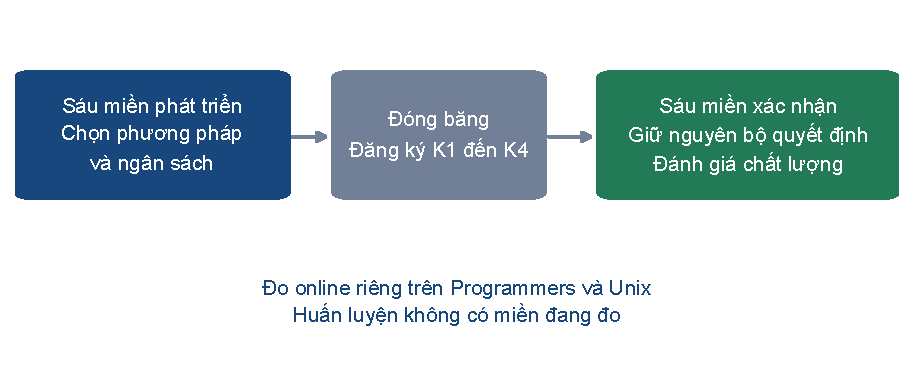
\includegraphics[width=\textwidth]{evaluation_protocol.pdf}
\caption{Quan hệ giữa phát triển, đóng băng và xác nhận. Nhánh online trên Programmers/Unix sử dụng mô hình được học không có miền đang đo, nên giữ vai trò riêng với xác nhận chất lượng trên sáu miền mới.}
\label{fig:protocol}
\end{figure}

Giao thức xác nhận được ghi nhận trước khi thu thập dữ liệu của sáu miền giữ lại. Hồ sơ chốt phương pháp, ngân sách và bốn giả thuyết K1 đến K4. Việc đăng ký không làm mất các giới hạn của nghiên cứu, nhưng giúp phân biệt kết quả kiểm chứng giả thuyết có trước với những nhận xét được hình thành sau khi đã biết số liệu.

Trên miền xác nhận, bộ quyết định v2 được giữ nguyên nhưng hệ thống có sử dụng truy vấn không nhãn để thích nghi với đặc điểm của miền và xác định chính sách vận hành. Đây là một điều kiện của phép đánh giá. Vì vậy, báo cáo phân biệt việc không dùng nhãn miền xác nhận để học lại mô hình với việc hoàn toàn chưa tiếp cận dữ liệu của miền đó.

\section{Các phương pháp đối chứng}
Đối chứng được tổ chức theo câu hỏi nghiên cứu. BM25 và Dense cho thấy chất lượng của từng nguồn truy xuất. \Pstar{} cho biết nhánh rẻ thực sự cải thiện được bao nhiêu so với BM25. \Hstar{} là mốc chất lượng và chi phí khi luôn sử dụng cả hai nguồn. \Rstar{} mã hóa truy vấn nhưng chỉ chấm lại các ứng viên BM25, nên kiểm tra một hướng tiết kiệm khác với bỏ qua encoder.

Để đánh giá khả năng lựa chọn, BM25-margin dùng mức khác biệt giữa các kết quả đầu danh sách làm quy tắc đơn giản không học. Lựa chọn ngẫu nhiên được thực hiện nhiều lần để giảm ảnh hưởng của một lần chọn tình cờ. Đối chứng oracle biết trước nhánh nào mang lại lợi ích lớn hơn cho từng truy vấn. Vì cần nhãn liên quan để đưa ra lựa chọn, oracle chỉ dùng để chỉ ra khoảng cải thiện còn có thể đạt được trong đánh giá, không phải phương pháp phục vụ truy vấn mới.

PE-GH v1 được giữ theo giao thức cũ, sử dụng mô hình ngữ nghĩa MiniLM \cite{minilm2020} và được lựa chọn bằng dữ liệu có nhãn trong từng miền. V2 thay đổi cả mô hình ngữ nghĩa, nhánh truy xuất và mục tiêu học. Vì vậy, so sánh v2 với v1 đánh giá mức tiến bộ của toàn hệ thống. Những khác biệt giữa hai phiên bản không cho phép quy toàn bộ chênh lệch kết quả cho riêng bộ quyết định.

Hai đối chứng dựa trên công trình trước được bổ sung sau phân tích chính. Một đối chứng dùng BERT \cite{bert2019} theo hướng lựa chọn của Arabzadeh, còn đối chứng LiteGator đại diện cho cách ra quyết định có chi phí thấp. Cả hai được điều chỉnh để cùng lựa chọn giữa \Pstar{} và \Hstar{} trên dữ liệu của đề tài. Những điều chỉnh về nhiệm vụ và mục tiêu dự báo thuộc cách áp dụng của nhóm, nên phần đối chiếu được xem là thăm dò, không phải tái lập nguyên vẹn kết quả công bố của hai bài báo.

Trong so khớp ngân sách, mọi bộ quyết định được dùng đúng cùng số lượt Dense trên mỗi phần dữ liệu và mỗi miền. Trong phép đo chi phí thăm dò, mô hình được lựa chọn mà không dùng miền đang đo. Những điều kiện chung về nhánh, dữ liệu và ngân sách giúp phép so sánh nhất quán hơn. Tuy nhiên, BERT chưa được khảo sát nhiều phương án như hai bộ quyết định nhẹ do chi phí phát triển cao hơn, nên kết quả vẫn có giới hạn về mức độ cân bằng giữa các đối chứng.

\section{Thước đo và nguyên tắc kiểm định}
Chất lượng chính được đo bằng \ndcg{} \cite{ndcg2002}. Thước đo phản ánh việc đưa các tài liệu liên quan lên những vị trí đầu, là phần danh sách có ý nghĩa trực tiếp đối với người dùng. Điểm tổng hợp chính là trung bình macro theo miền: trước hết tính trung bình truy vấn trong từng miền, sau đó lấy trung bình các miền với trọng số bằng nhau. Cách tổng hợp này tránh để miền TeX có nhiều truy vấn quyết định phần lớn kết quả gộp.

Các so sánh chất lượng được thực hiện trên cùng truy vấn để hạn chế ảnh hưởng của khác biệt dữ liệu \cite{smucker2007,urbano2019}. Khoảng tin cậy được ước lượng bằng lấy mẫu lại, có xét các nhóm truy vấn và vai trò ngang nhau của từng miền. Khoảng này mô tả bất định của kết quả trên dữ liệu đã đánh giá; nó chưa bao gồm đầy đủ biến động từ việc học lại mô hình, lựa chọn phương án hoặc chuyển sang một tập miền hoàn toàn khác.

K1 kiểm tra bộ quyết định v2 tốt hơn BM25-margin ở cùng ngân sách 50\%. K2 kiểm tra PE-GH ở ngân sách vận hành 80\% không kém \Hstar{} quá 0,01. K3 kiểm tra v2 tốt hơn v1 ở mức toàn hệ thống. K4 kiểm tra v2 tốt hơn lựa chọn ngẫu nhiên ở cùng ngân sách 50\%. Bốn phép kiểm định sử dụng p-value một phía và hiệu chỉnh Holm \cite{holm1979} với mức sai lầm toàn họ 0,05 theo giao thức đã đăng ký.

Với K2, kết luận không kém được chấp nhận khi bằng chứng thống kê cho thấy mức suy giảm chất lượng chưa vượt biên 0,01 đã xác định trước. Tiêu chí này cho phép một mất mát nhỏ, nên không đồng nghĩa hai phương pháp có chất lượng bằng nhau. Trong những so sánh thông thường khác, khoảng tin cậy chứa 0 chỉ cho biết chưa phát hiện khác biệt có ý nghĩa thống kê theo cách đánh giá đang dùng; điều đó cũng chưa chứng minh hai phương pháp tương đương.

Các đường cong ngân sách, AUC, kết quả từng miền và đối chiếu BERT/LiteGator bổ sung ngữ cảnh cho kết quả chính. Những phân tích ngoài K1 đến K4 được xem là mô tả hoặc thăm dò và không được gán hiệu chỉnh Holm của bốn giả thuyết đã đăng ký.

\section{Điều kiện đo chi phí truy xuất}
Các phương pháp được đo trên cùng một máy sử dụng CPU, trong điều kiện mỗi lần phục vụ một truy vấn và hệ thống đã sẵn sàng hoạt động. Thời gian được tính từ khi bắt đầu xử lý truy vấn đến khi có danh sách kết quả, bao gồm cả chi phí của bộ quyết định và phần truy xuất được lựa chọn. Cách đo này kiểm tra lợi ích thực tế của chính sách, thay vì suy ra thời gian tiết kiệm chỉ từ tỷ lệ bỏ qua Dense.

Phép đo chính bao gồm 97.400 yêu cầu trên 1.948 truy vấn, còn phiên đối chiếu thăm dò bao gồm 126.620 yêu cầu. Các phương pháp trong từng phiên dùng cùng tập truy vấn và được đo lặp lại để giảm tác động của dao động thời gian xử lý. Kết quả trả về trong lúc đo cũng được đối chiếu với kết quả đánh giá chất lượng để bảo đảm phép so sánh chi phí vẫn gắn với cùng hành vi truy xuất.

Độ trễ trung bình, p95, thời gian CPU và bộ nhớ đỉnh được báo cáo cùng tỷ lệ Dense thực tế. Khoảng tin cậy có xét việc cùng một truy vấn được đo nhiều lần. Mức giảm chi phí chỉ được tính so với đối chứng trong cùng phiên, nhằm hạn chế ảnh hưởng của khác biệt điều kiện đo.
